\documentclass[a4paper, 10pt]{article}
\usepackage{helvet}
\renewcommand{\familydefault}{\sfdefault}
\usepackage{pgf}
\usepackage{eurosym}
\usepackage{graphicx}
\usepackage{wasysym}
\usepackage{hyperref}
\usepackage{listings}
\usepackage{pxfonts}
\usepackage{verbatim}
\usepackage{color}
\usepackage{xcolor}
\usepackage{wrapfig}
\usepackage{enumitem}
\usepackage{booktabs}
\usepackage{gensymb}
\usepackage{tabularx}
\usepackage{currfile}

\hypersetup{
    bookmarks=true,         % show bookmarks bar?
    unicode=true,          % non-Latin characters in Acrobat’s bookmarks
    pdftoolbar=true,        % show Acrobat’s toolbar?
    pdfmenubar=true,        % show Acrobat’s menu?
    pdffitwindow=true,     % window fit to page when opened
    pdftitle={Assessments},    % title
    pdfauthor={Paul Vesey},     % author
    pdfsubject={I.C.T. Building Information Modelling},   % subject of the document
    pdfcreator={},   % creator of the document
    pdfproducer={xelatex}, % producer of the document
    pdfkeywords={'Graphics' }, % list of keywords
    pdfnewwindow=true,      % links in new PDF window
    colorlinks=true,       % false: boxed links; true: colored links
    linkcolor=violet,          % color of internal links (change box color with linkbordercolor)
    citecolor=magenta,        % color of links to bibliography
    filecolor=red,      % color of file links
    urlcolor=blue           % color of external links
}

\setlength\parindent{0pt}
\begin{document}

\lstset{language=HTML,
				basicstyle=\small,
				breaklines=true,
        numbers=left,
        numberstyle=\tiny,
        showstringspaces=false,
        aboveskip=-20pt,
        frame=leftline
        }
				
\begin{figure}
	\centering
	
\includegraphics[width=0.5\linewidth]{./Assignments/img/LITlogo}
\end{figure}


\begin{tabularx}{\textwidth}{ |l|X| }
	\hline
	\textbf{Subject:} & COMP06051-ICT \& BIM\\
	\textbf{Course:} & BEng in Civil Engineering\\
	\textbf{Session:} & Autumn 2022\\
	\textbf{Lecturer:} & Paul Vesey \footnotesize{BEng, MIE, HDip}\\
	\textbf{Filename:} & \currfilebase\\
	\hline
\end{tabularx}



\vspace{0.25cm}	
	
\begin{flushleft}
\Large\textbf{Assignment 1 (10\% of 40\%)- Microsoft Excel}\\
\end{flushleft}

In this assignment you are required to create a collection of Spreadsheets, within a single Microsoft Excel File, for the calculation of various properties of 2-dimensional shapes.  The key deliverables for this project are:

\begin{itemize}
	\item Fully working, annotated, and validated Microsoft Excel Spreadsheets
\end{itemize}

\textbf{Senario}\\


Attached to this specification you will find an extract from the NCEES Fundamentals of Engineering Reference Handbook V9.2, pages 65 to 67 inclusive.  You are required to create a single Microsoft Excel file with multiple sheets that will run the calculations of the formulae shown in the extract.  Please note that you are only required to create formulae for the Area, Centroid and Area Moment of Inertia only.  Radius of Gyration and Product of Inertia formulae are not required.  You spreadsheets should contain information that has shared characteristics, such as the shape or calculated result.  Your calculation areas should include a diagram and appropriate annotation for input and output cells.


\vspace{.5cm}

\textbf{Suggested Approach}

\begin{itemize}
	\item Select an appropriate grouping methodology
	\item Using the snipping tool, place diagrams into sheets as necessary
	\item Setup labels for each of the input and output parameters
	\item Create and test all formulae and intermediate results as appropriate
\end{itemize}

\textbf{Validation}\\
You should validate (test) your spreadsheets with a varity of data to ensure that your sheet behaves as expected, and returns results as expected.  You are required to submit a validation version of your spreadsheets with the data shown in Figures \ref{fig:ass2img1} to \ref{fig:ass2img3}.  This validation spreadsheet will be used to cross check your results.

\begin{figure}
	\centering
	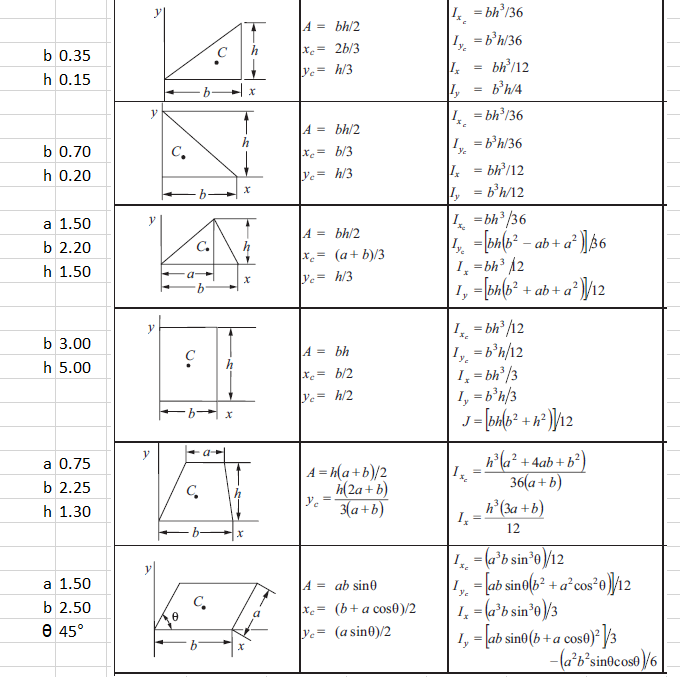
\includegraphics[width=1.0\linewidth]{img/Ass2Img1}
	\caption{Extract from page 65}
	\label{fig:ass2img1}
\end{figure}

\begin{figure}
	\centering
	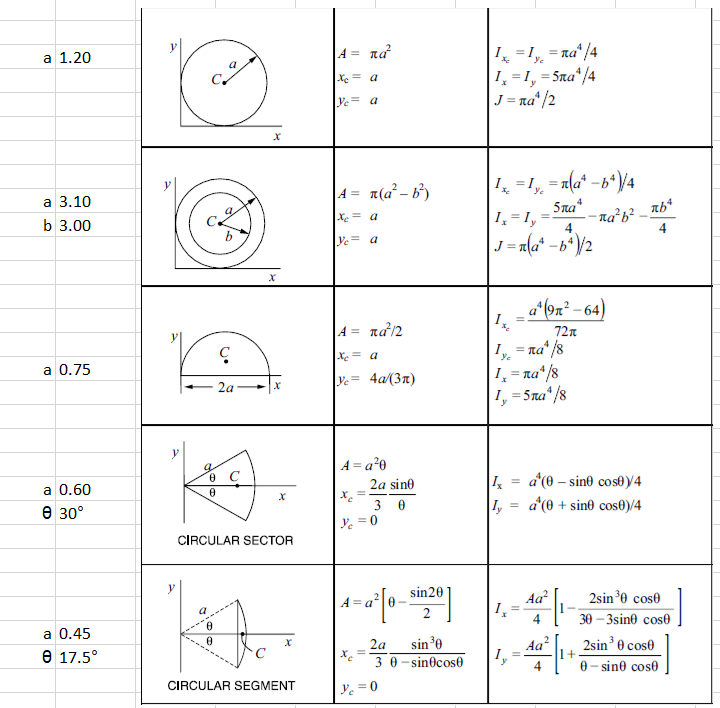
\includegraphics[width=1.0\linewidth]{img/Ass2Img2}
	\caption{Extract from page 66}
	\label{fig:ass2img2}
\end{figure}

\begin{figure}
	\centering
	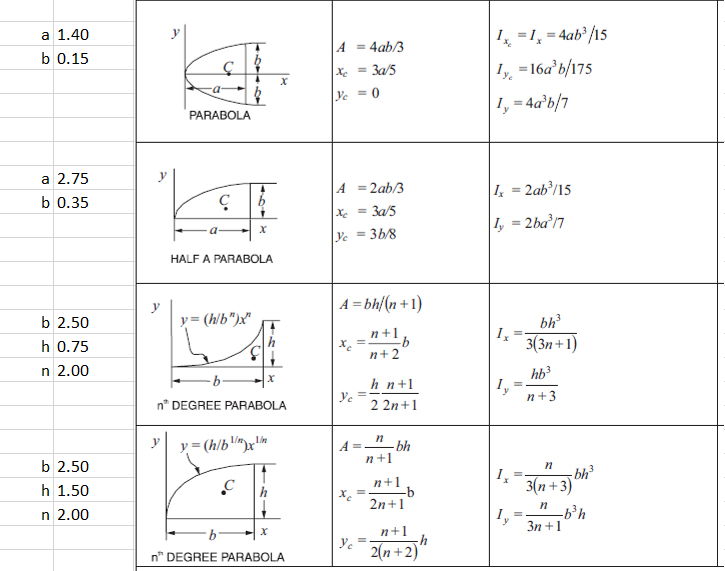
\includegraphics[width=1.0\linewidth]{img/Ass2Img3}
	\caption{Extract from page 67}
	\label{fig:ass2img3}
\end{figure}



\newpage


\textbf{Submission}\\
Your completed assignment comprising all computer files are to be zipped into a single file and uploaded to Moodle on or before the date and time indicated.  Key components of the submission are:
\begin{itemize}
	\item Fully working Excel file (no input data)with all necessary diagrams, formulas and annotations (.xlsx)
	\item File as above, validated with test data as provided (.xlsx)
\end{itemize}




\textbf{Late Submission}\\
Failure to submit your assignment on or before the date and time indicated on Moodle will result in a penalty of 5\% per day or part thereof.

\vspace{0.5cm}
\textbf{Marking Scheme}

\begin{table}[h!]
     \begin{center}
     \begin{tabular}{p{9cm}  p{2cm} }
     \toprule
      \textbf\large{Element} & \textbf\large{Proportion} \\ 
    \cmidrule(r){1-1}\cmidrule(lr){2-2}
      \textbf{MS Excel Spreadsheet, Annotations and Diagrams } & \textbf{70\%}\\
      \textbf{Validation Test Spreadsheet} & \textbf{30\%}\\
      \\ \bottomrule
      \end{tabular}
      \label{tbl:markSchemeAsmt3}
      \end{center}
 \end{table}


\end{document}